%% Elektrotechnik Workshop - Messaufzeichnung und regenerative Energieerzeugung
%% Dokumentationsvorlage
%% Geschrieben von Benjamin Hoffmann am 08.11.2012
%% (c) Lichttechnisches Institut (LTI), Karlsruher Institut für Technologie



\documentclass[11pt,ngerman]{scrartcl}
\usepackage{newcent}
\renewcommand{\familydefault}{\sfdefault}
\usepackage[T1]{fontenc}
\usepackage[latin9]{inputenc}
\usepackage[a4paper]{geometry}
\geometry{verbose,tmargin=25mm,bmargin=2.5cm,lmargin=2.5cm,rmargin=2cm,headheight=0.5cm,headsep=1cm,footskip=0.5cm}
\usepackage{fancyhdr}
\pagestyle{fancy}
\setlength{\parskip}{\smallskipamount}
\setlength{\parindent}{0pt}
\usepackage{color}
\usepackage{array}
\usepackage{multirow}
\usepackage{graphicx}
\usepackage{setspace}
\setstretch{1.3}

\makeatletter

%%%%%%%%%%%%%%%%%%%%%%%%%%%%%% LyX specific LaTeX commands.
%% Because html converters don't know tabularnewline
\providecommand{\tabularnewline}{\\}

%%%%%%%%%%%%%%%%%%%%%%%%%%%%%% User specified LaTeX commands.
\usepackage{colortbl}
\usepackage[framed,numbered,autolinebreaks,useliterate]{mcode}
%% Farbdefinitionen
\definecolor{mintgreen}{rgb}{0.6,0.73,0.38}
\definecolor{dunkelblau}{rgb}{0.12,0.28,0.49}
\definecolor{softblue}{rgb}{0.31,0.51,0.741}

%%Kopf und Fusszeile

\makeatother

\usepackage{babel}
\begin{document}
\newgeometry{left=22mm,right=15mm,top=30mm,bottom=10mm}

\noindent %
\begin{tabular}{cc}
\begin{tabular}{c}

\includegraphics[width=4cm]{KITLogo.pdf}\tabularnewline
\end{tabular} & %
\begin{tabular}{ll}
Lichttechnisches & Institut f�r Elektroenergiesysteme \tabularnewline
Institut (LTI) & und Hochspannungstechnik (IEH)\tabularnewline
\textit{M.Sc. Dipl.-Ing.}  & \textit{Dipl.-Ing.}\tabularnewline
\textit{Karsten H�hre} & \textit{Sebastian K�nig}\tabularnewline
\end{tabular}\tabularnewline
\multicolumn{2}{c}{\textbf{\huge \medskip{}
}}\tabularnewline
\end{tabular}

\begin{singlespace}
\noindent \begin{center}
\Huge\color{softblue}\textsf{\textbf{Workshop Elektro und Informationstechnik}}
\par\end{center}

\noindent \begin{center}
\LARGE\color{softblue}\textsf{\textbf{Messwertaufzeichnung und regenerative Energieerzeugung}}
\par\end{center}


\noindent \begin{center}
\textbf{\huge D}\textbf{\Large OKUMENTATION}\textbf{\LARGE{} }
\par\end{center}{\LARGE \par}
\end{singlespace}

\noindent \begin{center}
\textcolor{black}{\Large Gruppe: {[}Gruppenname{]}}
\par\end{center}{\Large \par}

\noindent \begin{center}
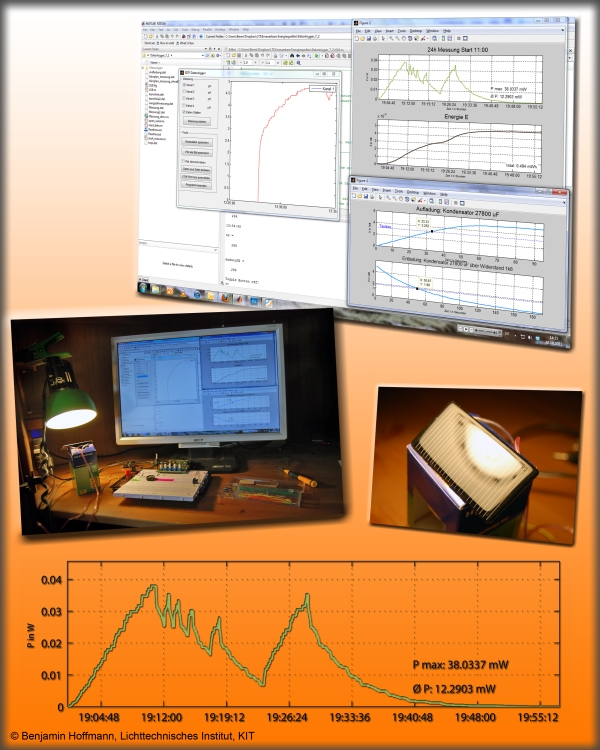
\includegraphics[height=8cm]{Titelbild}
\par\end{center}

\noindent \begin{center}
\begin{tabular}{|c|c|c|c|c|}
\hline
\textit{\textcolor{black}{\small \cellcolor{softblue} Vorname }}%
\begin{tabular}{c}
\bigskip{}\tabularnewline
\end{tabular} & \textit{\textcolor{black}{\small \cellcolor{softblue}Nachname}} & \textit{\textcolor{black}{\small \cellcolor{softblue}Matrikelnr.}} & \textit{\textcolor{black}{\small \cellcolor{softblue}}}\textit{\textcolor{black}{\footnotesize u-Account}} & \textit{\textcolor{black}{\small \cellcolor{softblue}E-Mail}}\tabularnewline
\hline
\hline
\multirow{2}{*}{{\small {[}name1{]}}} & \multirow{2}{*}{{\small {[}vorname1{]}}} & \multirow{2}{*}{{\small {[}manr1{]}}} & \multirow{2}{*}{{\small {[}uxxxx1{]}}} & \multirow{2}{*}{{[}Name.Vorname@student.kit.edu1{]}}\tabularnewline
 &  &  &  & \tabularnewline
\hline
\multirow{2}{*}{{\small {[}name2{]}}} & \multirow{2}{*}{{\small {[}vorname2{]}}} & \multirow{2}{*}{{\small {[}manr2{]}}} & \multirow{2}{*}{{\small {[}uxxxx2{]}}} & \multirow{2}{*}{{[}Name.Vorname@student.kit.edu2{]}}\tabularnewline
 &  &  &  & \tabularnewline
\hline
\multirow{2}{*}{{\small {[}name3{]}}} & \multirow{2}{*}{{\small {[}vorname3{]}}} & \multirow{2}{*}{{\small {[}manr3{]}}} & \multirow{2}{*}{{\small {[}uxxxx3{]}}} & \multirow{2}{*}{{[}Name.Vorname@student.kit.edu3{]}}\tabularnewline
 &  &  &  & \tabularnewline
\hline
\multirow{2}{*}{{\small {[}name4{]}}} & \multirow{2}{*}{{\small {[}vorname4{]}}} & \multirow{2}{*}{{\small {[}manr4{]}}} & \multirow{2}{*}{{\small {[}uxxxx4{]}}} & \multirow{2}{*}{{[}Name.Vorname@student.kit.edu4{]}}\tabularnewline
 &  &  &  & \tabularnewline
\hline
\end{tabular}
\par\end{center}

\noindent \thispagestyle{empty}\newpage{}

\lhead{\textsf{\textbf{Workshop ETIT}} }		%% Kopfzeile links
\chead{\textsf{Kurs 1}} 	%% Kopfzeile mitte
\rhead{\textsf{WS 2012/13} }	%% Kopfzeile rechts
\lfoot{\textsf{Messwertaufzeichnung \& regenerative Energieerzeugung}} 		%% Fu�zeile links
\cfoot{ } 		%% Fu�zeile mitte
\rfoot{\textsf{Seite: \thepage}}	%% Fu�zeile rechts und dies ist Seite:

\renewcommand{\headrulewidth}{0.5pt}
\renewcommand{\footrulewidth}{0.5pt}

\setcounter{page}{1}

\noindent \tableofcontents{}

\noindent \newpage{}


\part{\noindent \textcolor{black}{Verschiedene Strahlungsquellen }}
Die folgenden Erkl�rungen sollen Ihnen die Verkn�pfung von MATLAB und Latex erleichtern. Sie sollen in Ihrer Ausarbeitung nicht mehr enthalten sein.

\section{Einbinden von MATLAB-Skripten}

Ein MATLAB-Skript kann mit dem Befehl
\begin{verbatim}
\lstinputlisting{Beispiel.m}
\end{verbatim}
eingebunden werden. Ersetzen Sie einfach den Dateinamen \textit{Beispiel.m} durch Pfad und Namen Ihres Skripts. Die Ausgabe des Skripts stellt sich wie folgt dar.
\lstinputlisting{Beispiel.m}

Weitere Informationen zu dem Paket \textit{mcode.sty} finden Sie innerhalb der Datei, welche Sie mit jedem Textbearbeitungsprogramm �ffnen k�nnen.

\section{Einbindung von MATLAB-Matrizen}
Das kleine MATLAB-Programm \textit{Beispiel.m} zeigt au�erdem die Verwendung des Befehls \textit{latex.m}. F�gen Sie zu dessen Verwendung die Datei \textit{latex.m} in das MATLAB-Verzeichnis ein bzw. stellen Sie �ber \textit{Set Path} sicher, dass MATLAB den Ordner, in dem sich die Datei befindet, kennt. Mit \textit{latex(M)} k�nnen Sie dann die Matrix M im Befehlsfenster von MATLAB in der Form ausgeben lassen, dass Sie sie direkt in Ihr Latex-File kopieren k�nnen, wie folgendes Beispiel zeigt.

\begin{verbatim}
\begin{table}
\centering
\begin{tabular}{|l|l|l|}
\hline
Zeit&sin-Funktion&cos-Funktion\\
\hline

$0.00000$ & $0.00000$ & $1.0000$ \\
$1.0000$ & $0.84147$ & $0.54030$ \\
$2.0000$ & $0.90930$ & $-0.41615$ \\
$3.0000$ & $0.14112$ & $-0.98999$ \\
$4.0000$ & $-0.75680$ & $-0.65364$ \\
$5.0000$ & $-0.95892$ & $0.28366$ \\
$6.0000$ & $-0.27942$ & $0.96017$ \\
\hline
\end{tabular}
\caption{Tabelle erzeugt mit Beispiel.m} \label{Beispieltabelle}
\end{table}
\end{verbatim}

Die gezeigte Sequenz erzeugt dann Tabelle \ref{Beispieltabelle}.
\begin{table}[!h]
\centering
\begin{tabular}{|l|l|l|}
\hline
Zeit&sin-Funktion&cos-Funktion\\
\hline
$0.00000$ & $0.00000$ & $1.0000$ \\
$1.0000$ & $0.84147$ & $0.54030$ \\
$2.0000$ & $0.90930$ & $-0.41615$ \\
$3.0000$ & $0.14112$ & $-0.98999$ \\
$4.0000$ & $-0.75680$ & $-0.65364$ \\
$5.0000$ & $-0.95892$ & $0.28366$ \\
$6.0000$ & $-0.27942$ & $0.96017$ \\

\hline
\end{tabular}
\caption{Tabelle erzeugt mit Beispiel.m} \label{Beispieltabelle}
\end{table}

\part{\noindent Langzeitmessung}


\part{\noindent Energiespeicherung}





\part{\noindent Leistungsvergleich}



\end{document}
